\documentclass[17pt,a4paper]{extarticle}
\usepackage[utf8]{inputenc}
\usepackage[T1]{fontenc}
\usepackage{lmodern}
\usepackage[margin=1in]{geometry}
\usepackage{amsmath,amssymb}
\usepackage{graphicx}
\usepackage[colorlinks=true,linkcolor=blue,citecolor=blue,urlcolor=blue]{hyperref}
\usepackage{caption}
\usepackage{booktabs}
\usepackage[thai]{babel}
\usepackage{tikz}
\newcommand{\mycorner}{10pt}
\tikzset{
    roundedimg/.style={
        rounded corners=\mycorner, % Corner radius
    }
}
\title{A Sample LaTeX Document}
\author{Your Name}
\date{\today}




% 1. Load fontspec for font management
\usepackage{fontspec}

% 2. Use babel to handle Thai language rules and line breaking
\usepackage[thai]{babel}

% 3. Specify your system's Thai font
\setmainfont{TH Sarabun New}


\begin{document}

\maketitle

\begin{abstract}
	ทดสอบการพิมพ์ภาษาไทยใน VS Code ด้วย LuaLaTeX	This is a short  ddd example LaTeX document generated to get you started. Replace sections below with your content.
\end{abstract}


\noindent เข้าในเวปดังกล่าวแล้วคลิกที่ปุ่มดาวน์โหลดเพื่อดาวน์โหลดระฆังบนโชในรูปแบบไฟล์ STL จากนั้นคุณสามารถใช้โปรแกรมการพิมพ์ 3 มิติที่คุณชื่นชอบเพื่อพิมพ์ระฆังบนโชของคุณเองได้ตามต้องการ


\begin{figure}[ht]
	\centering

	\begin{tikzpicture}

		\node[draw=none, rounded corners=\mycorner, inner sep=0pt, clip] (image) {
			% \includegraphics[width=0.5\textwidth]{example-image}
			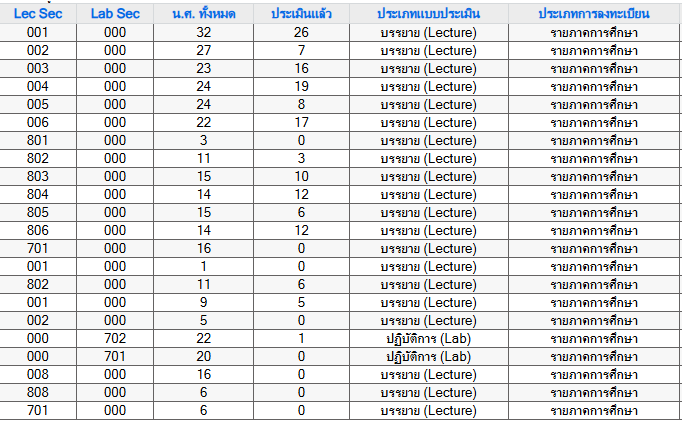
\includegraphics[width=0.8\textwidth]{2026-03-14-05-57-07.png}
		};

	\end{tikzpicture}
	\caption{}
\end{figure}
\section{Introduction}
This template demonstrates a minimal but useful structure: title, abstract, sections, an equation, a figure placeholder, and references.
ะฆังบนโชโดยทั่วไปทำมาจากทองสัมฤทธิ์ หล่อด้วยแม่พิมพ์แบบใช้ครั้งเดียว โดยทั่วไปมักเสริมและประดับด้วยปุ่มนูน เส้นแถบนูน และคำจารึก บนโชที่เก่าแก่ที่สุดในญี่ปุ่นสร้างขึ้นราว ค.ศ. 600 แม้ว่าระฆังใบนี้จะมีรูปแบบการออกแบบโดยรวมจะมีที่มาจากจีนยุคก่อนมากกว่า และมีคุณลักษณะบางประการร่วมกับระฆังจีนโบราณก็ตาม เสียงของระฆังบนโชมีลักษณะก้องกังวานและทะลุทะลวง จึงนำมาใช้บอกสัญญาณ บอกเวลา และแจ้งเตือน นอกจากนี้ยังเชื่อว่าเสียงของบนโชมีคุณสมบัติเหนือธรรมชาติ เป็นต้นว่า มีความเชื่อว่าเสียงระฆังนี้ได้ยินไปถึงนรก
\section{Math example}
Inline equation: $E=mc^2$. Display equation:
\begin{equation}
	\label{eq:sample}
	\nabla\cdot\mathbf{E} = \frac{\rho}{\varepsilon_0}
\end{equation}


\begin{figure}[ht]
	\centering
	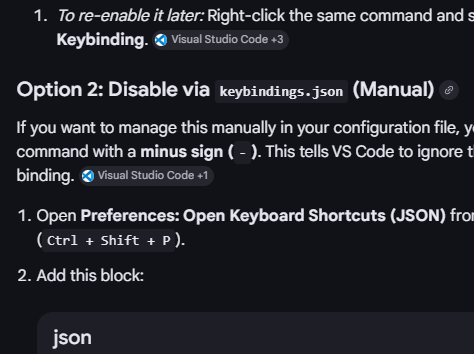
\includegraphics[width=0.8\textwidth]{2026-03-14-05-54-24.png}
	\caption{}
\end{figure}

\section{Figure example}
Place a figure in the project folder and update the filename below.
\begin{figure}[h]
	\centering
	% \includegraphics[width=0.6\textwidth]{example-image.png}
	\caption{Example figure (uncomment and set filename).}
	\label{fig:example}
\end{figure}

\section{Conclusion}
Summarize your findings here.

\section*{References}
\begin{thebibliography}{9}
	\bibitem{lamport94}
	Leslie Lamport,
	\emph{LaTeX: A Document Preparation System},
	Addison Wesley, 2nd edition, 1994.
\end{thebibliography}

\end{document}

